\documentclass[tikz, border=10pt]{standalone}
\usepackage{tikz}
\usetikzlibrary{shapes, shadows, calc, positioning, decorations.pathreplacing}

% Define colors
\definecolor{GeoskanBlue}{RGB}{0, 89, 166}
\definecolor{GeoskanOrange}{RGB}{255, 100, 0}
\definecolor{GeoskanBlack}{RGB}{30, 30, 30}
\definecolor{GeoskanSilver}{RGB}{200, 200, 200}
\definecolor{GeoskanGuard}{RGB}{220, 230, 240}
\definecolor{GeoskanGreen}{RGB}{0, 200, 0}
\definecolor{GeoskanRed}{RGB}{200, 0, 0}

\begin{document}
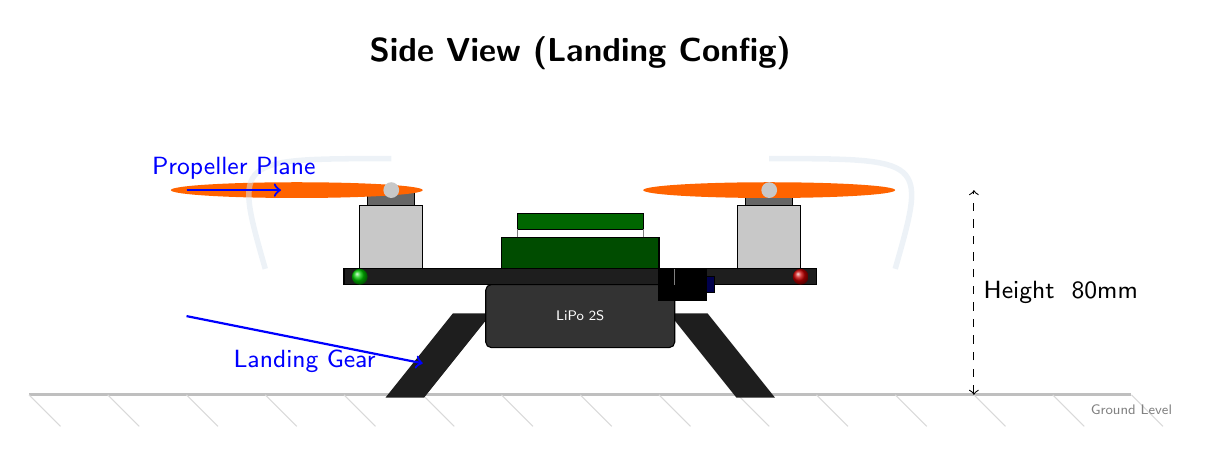
\begin{tikzpicture}[scale=2]

    % --- Ground ---
    \draw[line width=1pt, color=gray!50] (-3.5, 0) -- (3.5, 0);
    \foreach \x in {-3.5, -3, ..., 3.5} {
        \draw[gray!30] (\x, 0) -- (\x+0.2, -0.2);
    }
    \node[anchor=north, gray, font=\sffamily\tiny] at (3.5, 0) {Ground Level};

    % --- Landing Legs (Simplified) ---
    % Front Legs
    \draw[line width=2pt, color=GeoskanBlack, fill=GeoskanBlack] (-1.2, 0) -- (-0.8, 0.5) -- (-0.6, 0.5) -- (-1.0, 0) -- cycle;
    \draw[line width=2pt, color=GeoskanBlack, fill=GeoskanBlack] (1.2, 0) -- (0.8, 0.5) -- (0.6, 0.5) -- (1.0, 0) -- cycle;
    
    % Rear Legs (Slightly smaller for perspective, but side view is mostly flat)
    % Just imply structure
    
    % --- Main Body (Battery + Frame) ---
    % Battery Hanging
    \draw[fill=black!80, rounded corners=2pt] (-0.6, 0.3) rectangle (0.6, 0.7);
    \node[white, font=\tiny\sffamily] at (0, 0.5) {LiPo 2S};

    % Frame Plate
    \draw[fill=GeoskanBlack] (-1.5, 0.7) rectangle (1.5, 0.8);
    
    % --- Motors ---
    % Left Motor
    \draw[fill=GeoskanSilver] (-1.4, 0.8) rectangle (-1.0, 1.2);
    \draw[fill=black!60] (-1.35, 1.2) rectangle (-1.05, 1.3); % Shaft base
    
    % Right Motor
    \draw[fill=GeoskanSilver] (1.0, 0.8) rectangle (1.4, 1.2);
    \draw[fill=black!60] (1.05, 1.2) rectangle (1.35, 1.3); % Shaft base

    % Center Electronics Stack
    \draw[fill=green!30!black] (-0.5, 0.8) rectangle (0.5, 1.0); % PCB 1
    \draw[fill=green!40!black] (-0.4, 1.05) rectangle (0.4, 1.15); % PCB 2 (Upper deck)
    \draw[gray] (-0.4, 1.0) -- (-0.4, 1.05); % Standoff
    \draw[gray] (0.4, 1.0) -- (0.4, 1.05);   % Standoff

    % --- Propellers (Side View) ---
    % Left Prop (Orange)
    \fill[GeoskanOrange] (-1.8, 1.3) ellipse (0.8 and 0.05);
    \fill[GeoskanSilver] (-1.2, 1.3) circle (0.05); % Nut

    % Right Prop (Orange)
    \fill[GeoskanOrange] (1.2, 1.3) ellipse (0.8 and 0.05);
    \fill[GeoskanSilver] (1.2, 1.3) circle (0.05); % Nut

    % --- Guard (Side View Projection) ---
    \draw[GeoskanGuard, line width=2pt, opacity=0.5] (-2.0, 0.8) .. controls (-2.2, 1.5) .. (-1.2, 1.5);
    \draw[GeoskanGuard, line width=2pt, opacity=0.5] (2.0, 0.8) .. controls (2.2, 1.5) .. (1.2, 1.5);

    % --- Camera Module (Front/Side) ---
    \draw[fill=black] (0.5, 0.6) rectangle (0.8, 0.8); % Camera body
    \draw[fill=blue!30!black] (0.8, 0.65) rectangle (0.85, 0.75); % Lens
    \draw[gray] (0.6, 0.8) -- (0.6, 0.7); % Mount

    % --- LED Indicators ---
    % Green LED (Armed/Ready)
    \shade[ball color=GeoskanGreen] (-1.4, 0.75) circle (0.05);
    \shade[ball color=GeoskanRed] (1.4, 0.75) circle (0.05);

    % --- Annotations ---
    \draw[->, thick, blue] (-2.5, 1.3) -- node[above, font=\small\sffamily] {Propeller Plane} (-1.9, 1.3);
    \draw[->, thick, blue] (-2.5, 0.5) -- node[below, font=\small\sffamily] {Landing Gear} (-1.0, 0.2);
    
    % Altitude Indicator
    \draw[<->, dashed] (2.5, 0) -- (2.5, 1.3) node[midway, right, font=\small\sffamily] {Height ~80mm};

    % Title
    \node[font=\large\bfseries\sffamily, anchor=south] at (0, 2.0) {Side View (Landing Config)};

\end{tikzpicture}
\end{document}
